\clearpage
\begin{textbox}{\href{https://compneuro.neuromatch.io/tutorials/W0D5_Statistics/student/W0D5_Tutorial1.html}{Statistics (W0D5T1)} - Probability Distributions}
\begin{subbox}{subbox}{Random Walk}
\scriptsize
Stochastic models can be used to create models of behaviour. As an example, imagine that a rat is placed inside a novel environment, a box. We could try and model its exploration behaviour by assuming that for each time step it takes a random uniformly sampled step in any direction (simultaneous random step in x direction and random step in y direction)

\centering
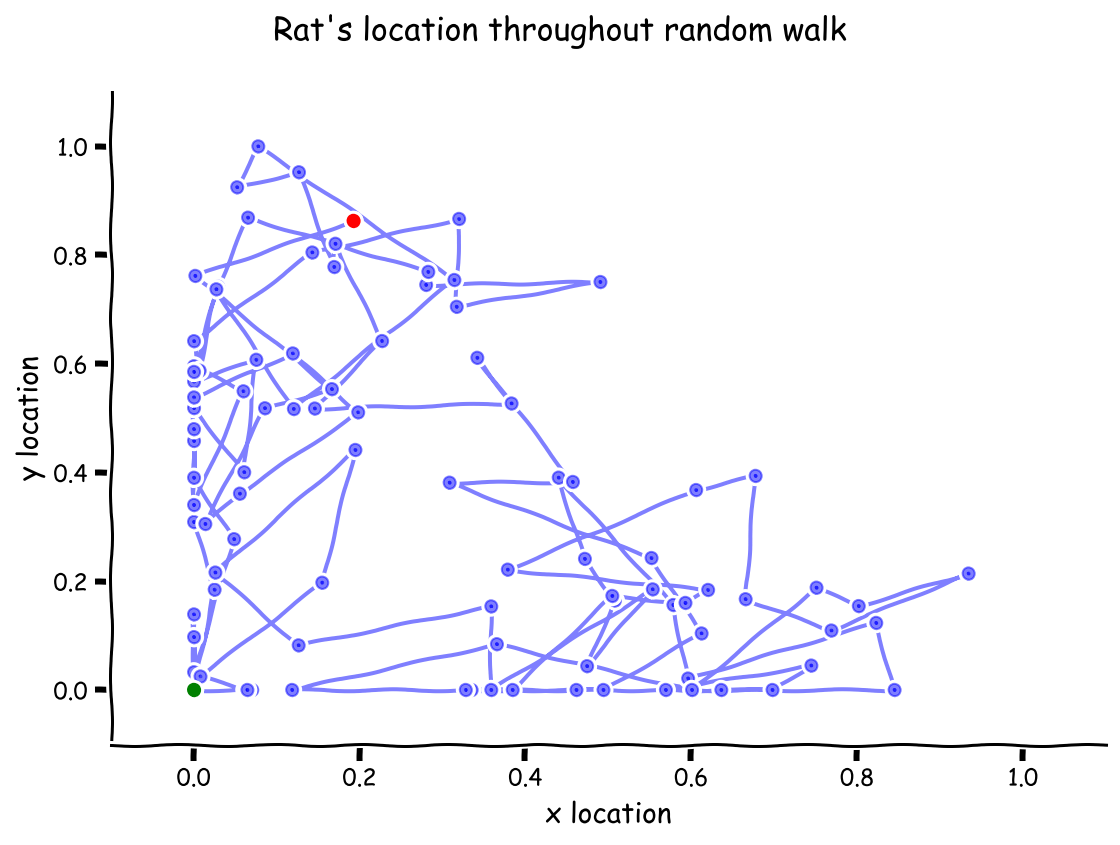
\includegraphics[scale=0.08]{Figures/PreCourse/SFigure1.png}
\end{subbox}

\begin{subbox}{subbox}{Discrete Distributions Differentiation}
\scriptsize{

A simple way to model random behaviour is with a single \textbf{Bernoulli trial}, that has two outcomes, {$Left, Right$}, with probability $P(Left)=p$ and $P(Right)=1-p$ as the two mutually exclusive possibilities (whether the rat goes down the left or right arm of the maze).

\textbf{The binomial distribution} simulates $n$ number of binary events, such as the $Left, Right$ choices of the random rat in the T-maze is given by:
\begin{align}
P(k|n,p) &= \left( \begin{array} \\n \\ k\end{array} \right) p^k (1-p)^{n-k} \\
\binom{n}{k} &= {\frac {n!}{k!(n-k)!}}
\end{align}

where, $p$ is the probability of turning left, $n$ is the number of binary events, or trials, and $k$ is the number of times the rat turned left. The term $\binom {n}{k}$ is the binomial coefficient.

\textbf{The Poisson distribution} is a 'point-process', meaning that it determines the number of discrete 'point', or binary, events that happen within a fixed space or time, allowing for the occurrence of a potentially infinite number of events. The Poisson distribution is specified by a single parameter $\lambda$ that encapsulates the mean number of events that can occur in a single time or space interval.
The formula for a Poisson distribution is: 
\begin{equation}
P(x)=\frac{\lambda^x e^{-\lambda}}{x!}
\end{equation}
where $\lambda$ is a parameter corresponding to the average outcome of $x$.
}
\end{subbox}
\end{textbox}
%%%%%%%%%%%%%%%%%%%%%%%%%%%%%%%%%%%%%%%%%%%%%%%%%
%%%%%%%%%%%%%%%%%%%%%%%%%%%%%%%%%%%%%%%%%%%%%%%%%
\begin{textbox}{\href{https://compneuro.neuromatch.io/tutorials/W0D5_Statistics/student/W0D5_Tutorial1.html}{Statistics (W0D5T1)} - Probability Distributions}
\begin{subbox}{subbox}{Continuous Distributions}
\scriptsize
We do not have to restrict ourselves to only probabilistic models of discrete events. 
While for discrete outcomes we can ask about the probability of an specific event ("what is the probability this neuron will fire 4 times in the next second"), this is not defined for a continuous distribution ("what is the probability of the BOLD signal being exactly 4.000120141..."). Hence we need to focus on intervals when calculating probabilities from a continuous distribution. 

If we want to make predictions about possible outcomes for a continuous distribution we can use the integral
\begin{equation} 
\int_{x_1}^{x_2} P(x) dx 
\end{equation}
where $P(x)$ is a probability density function.

\end{subbox}
\begin{subbox}{subbox}{Gaussian Distribution}
\scriptsize
The most widely used continuous distribution is probably the Gaussian (also known as Normal) distribution. It is extremely common across all kinds of statistical analyses. Because of the central limit theorem, many quantities are Gaussian distributed. Gaussians also have some nice mathematical properties that permit simple closed-form solutions to several important problems. 

The equation for a Gaussian probability density function is:

\begin{equation}
f(x;\mu,\sigma^2) = \mathcal{N}(\mu,\sigma^2) = \frac{1}{\sqrt{2\pi\sigma^2}}\exp\left(\frac{-(x-\mu)^2}{2\sigma^2}\right)
\end{equation}

where $\mu=-1$ is the mean, $\sigma=1$ is the variance and $x$ is the random variable for orientation (degrees). 


\centering
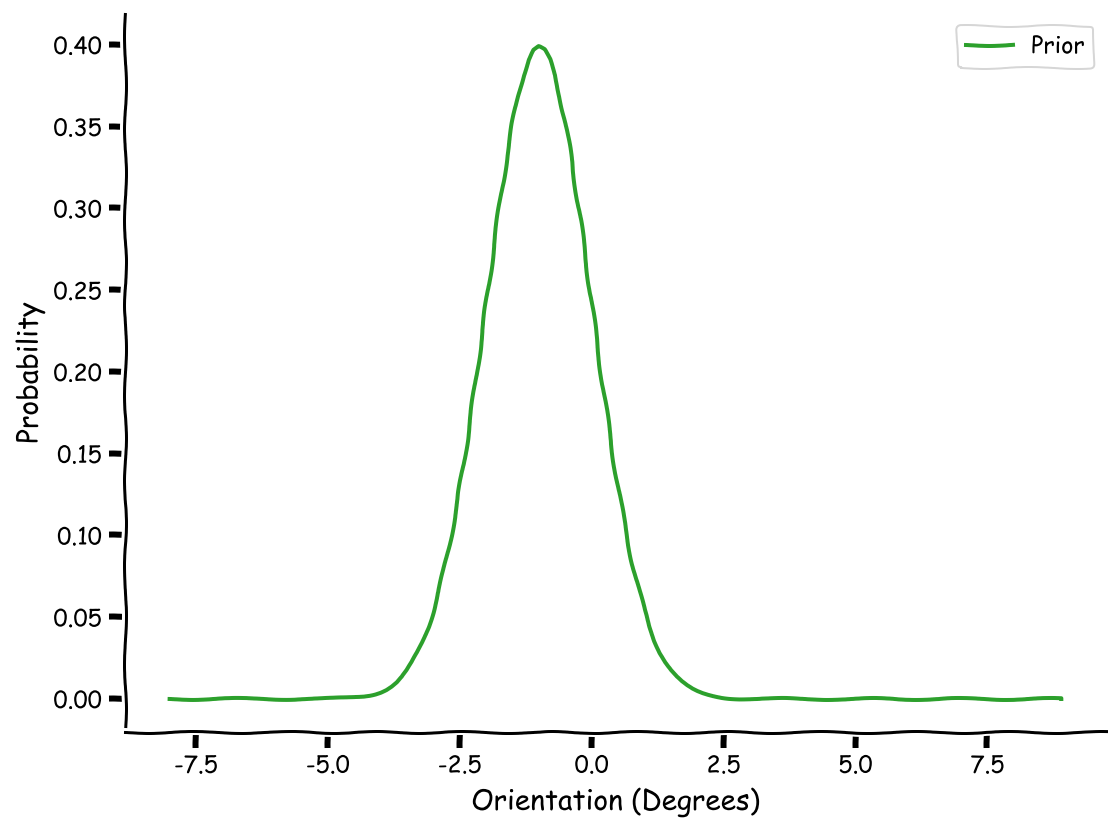
\includegraphics[scale=0.1]{Figures/PreCourse/SFigure2.png}

\end{subbox}
\end{textbox}
%%%%%%%%%%%%%%%%%%%%%%%%%%%%%%%%%%%%%%%%%%%%%%%%%
%%%%%%%%%%%%%%%%%%%%%%%%%%%%%%%%%%%%%%%%%%%%%%%%%
\begin{textbox}{\href{https://compneuro.neuromatch.io/tutorials/W0D5_Statistics/student/W0D5_Tutorial2.html}{Statistics (W0D5T2)} - Statistical Inference}
\begin{subbox}{subbox}{Basic Probability}
\scriptsize

Probability has to be in the range 0 to 1
$P(A) \in  [0,1] $

and the complementary can always be defined as
$$P(\neg A) = 1-P(A).$$
When we have two variables, the \textbf{conditional probability} of $A$ given $B$ is 
$$P (A|B) = P (A \cap B)/P (B)=P (A, B)/P (B)$$
while the \textbf{joint probability} of $A$ and $B$ is
$$P(A \cap B)=P(A,B) = P(B|A)P(A) = P(A|B)P(B) $$
We can then also define the process of \textbf{marginalisation} (for discrete variables) as 
$$P(A)=\sum P(A,B)=\sum P(A|B)P(B)$$ 
where the summation is over the possible values of $B$.

As an example if $B$ is a binary variable that can take values $B+$ or $B0$ then 
$$P(A)=\sum P(A,B)=P(A|B+)P(B+)+ P(A|B0)P(B0). $$

For continuous variables marginalization is given as 
$$P(A)=\int P(A,B) dB=\int P(A|B)P(B) dB.$$ 
\end{subbox}
\begin{subbox}{subbox}{Markov chains}
\scriptsize
The Markov property specifies that you can fully encapsulate the important properties of a system based on its current state at the current time, any previous history does not matter. It is memoryless.

As an example imagine that a rat is able to move freely between 3 areas: a dark rest area
($state=1$), a nesting area ($state=2$) and a bright area for collecting food ($state=3$). Every 5 minutes (timepoint $i$) we record the rat's location. We can use a **categorical distribution** to look at the probability that the rat moves to one state from another.

We can model this as a Markov chain, so the animal is only in one of the states at a time and can transition between the states.
We want to get the probability of each state at time $i+1$.
\begin{align*}
P(state_{i+1} = 1)=&\\ P(state_{i+1}=1|state_i=1)P(state_i = 1)  \\ +P(state_{i+1}=1|state_i=2)P(state_i = 2)  \\ +P(state_{i+1}=1|state_i=3)P(state_i = 3)
\end{align*}

\end{subbox}
\end{textbox}
%%%%%%%%%%%%%%%%%%%%%%%%%%%%%%%%%%%%%%%%%%%%%%%%%
%%%%%%%%%%%%%%%%%%%%%%%%%%%%%%%%%%%%%%%%%%%%%%%%%
\begin{textbox}{\href{https://compneuro.neuromatch.io/tutorials/W0D5_Statistics/student/W0D5_Tutorial2.html}{Statistics (W0D5T2)} - Statistical Inference}
\begin{subbox}{subbox}{Statistical inference and likelihood}
\scriptsize
If we do not know the parameters $\mu$, $\sigma$ that generated the data, we can try to \textbf{infer} which parameter values (given our model) gives the best (highest) likelihood. This is what we call statistical inference: trying to infer what parameters make our observed data the most likely or probable.

A generative model (such as the Gaussian distribution from the previous tutorial) allows us to make predictions about outcomes. 

After we observe $n$ data points, we can evaluate our model (and any of its associated parameters) by calculating the \textbf{likelihood} of our model having generated each of those data points $x_i$.

\begin{equation}
P(x_i|\mu,\sigma)=\mathcal{N}(x_i,\mu,\sigma)
\end{equation}

For all data points $\mathbf{x}=(x_1, x_2, x_3, ...x_n) $ we can then calculate the likelihood for the whole dataset by computing the product of the likelihood for each single data point.

\begin{equation}
P(\mathbf{x}|\mu,\sigma)=\prod_{i=1}^n \mathcal{N}(x_i,\mu,\sigma)
\end{equation}

While the likelihood may be written as a conditional probability ($P(x|\mu,\sigma)$), we refer to it as the \textbf{likelihood function}, $L(\mu,\sigma)$.  This slight switch in notation is to emphasize our focus: we use likelihood functions when the data points $\mathbf{x}$ are fixed and we are focused on the parameters.

Our new notation makes clear that the likelihood $L(\mu,\sigma)$ is a function of $\mu$ and $\sigma$, not of $\mathbf{x}$.


\end{subbox}
\begin{subbox}{subbox}{Maximum likelihood}
\scriptsize
Implicitly, by looking for the parameters that give the highest likelihood in the last section, we have been searching for the \textbf{maximum likelihood} estimate
\begin{equation}
(\hat{\mu},\hat{\sigma}) = \text{argmax}_{\mu,\sigma}L(\mu,\sigma) = \text{argmax}_{\mu,\sigma} \prod_{i=1}^n \mathcal{N}(x_i,\mu,\sigma).
\end{equation}

We want to do inference on this data set, i.e. we want to infer the parameters that most likely gave rise to the data given our model. Intuitively that means that we want as good as possible a fit between the observed data and the probability distribution function with the best inferred parameters. We can search for the best parameters manually by trying out a bunch of possible values of the parameters, computing the likelihoods, and picking the parameters that resulted in the highest likelihood. 

\end{subbox}
\end{textbox}
%%%%%%%%%%%%%%%%%%%%%%%%%%%%%%%%%%%%%%%%%%%%%%%%%
%%%%%%%%%%%%%%%%%%%%%%%%%%%%%%%%%%%%%%%%%%%%%%%%%
\begin{textbox}{\href{https://compneuro.neuromatch.io/tutorials/W0D5_Statistics/student/W0D5_Tutorial2.html}{Statistics (W0D5T2)} - Statistical Inference}
\begin{subbox}{subbox}{Bayesian Inference}
\scriptsize
For Bayesian inference we do not focus on the likelihood function $L(y)=P(x|y)$, but instead focus on the posterior distribution: 

\begin{equation}
P(y|x)=\frac{P(x|y)P(y)}{P(x)}
\end{equation}

which is composed of the **likelihood** function $P(x|y)$, the **prior** $P(y)$ and a normalising term $P(x)$ (which we will ignore for now).

While there are other advantages to using Bayesian inference (such as the ability to derive Bayesian Nets, see optional bonus task below), we will start by focusing on the role of the prior in inference.

\end{subbox}
\begin{subbox}{subbox}{Conjugate priors}
\scriptsize
Bayesian inference can be used for any likelihood distribution, but it is a lot more convenient to work with \textbf{conjugate} priors, where multiplying the prior with the likelihood just provides another instance of the prior distribution with updated values. 

For the binomial likelihood it is convenient to use the beta distribution as a prior

\begin{equation}
f(p;\alpha ,\beta )={\frac {1}{\mathrm {B} (\alpha ,\beta )}}p^{\alpha -1}(1-p)^{\beta -1}
\end{equation}

where $B$ is the beta function, $\alpha$ and $\beta$ are parameters, and $p$ is the probability of the rat turning left or right. The beta distribution is thus a distribution over a probability.

Given a series of Left and Right moves of the rat, we can now estimate the probability that the animal will turn left. Using Bayesian Inference, we use a beta distribution \textbf{prior}, which is then multiplied with the \textbf{likelihood} to create a \textbf{posterior} that is also a beta distribution, but with updated parameters. 

\centering
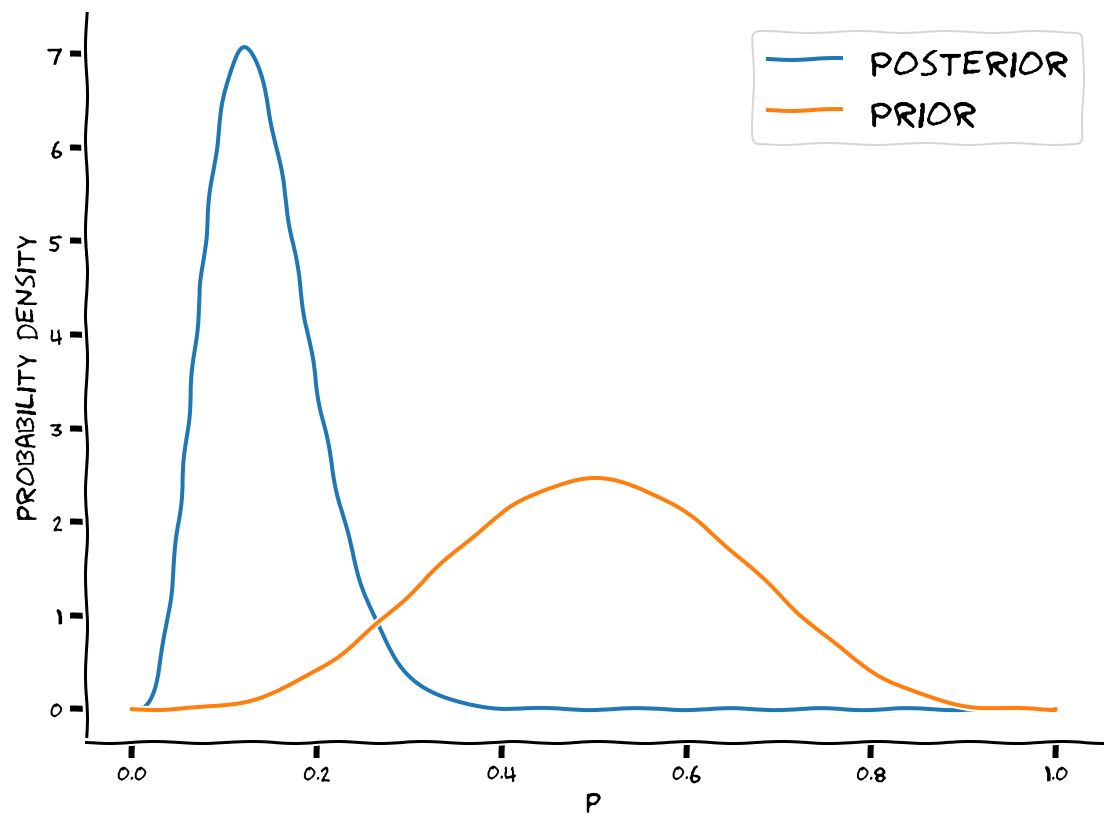
\includegraphics[scale=0.3]{Figures/PreCourse/SFigure3.png}

\end{subbox}
\end{textbox}